% !TeX program = lualatex
% TeX TXS-program:compile = txs:///lualatex/[-shell-escape]
%% Document based on `DEMO-TUDaThesis.tex' version 3.28 (2022/11/15),
%% A part of
%% TUDa-CI -- Corporate Design for TU Darmstadt
%%

\documentclass[
	ngerman,
	ruledheaders=section,%Ebene bis zu der die Überschriften mit Linien abgetrennt werden, vgl. DEMO-TUDaPub
	class=report,% Basisdokumentenklasse. Wählt die Korrespondierende KOMA-Script Klasse
	thesis={type=master},% Dokumententyp Thesis, für Dissertationen siehe die Demo-Datei DEMO-TUDaPhd
	accentcolor=9c,% Auswahl der Akzentfarbe
	custommargins=true,% Ränder werden mithilfe von typearea automatisch berechnet
	marginpar=false,% Kopfzeile und Fußzeile erstrecken sich nicht über die Randnotizspalte
	%BCOR=5mm,%Bindekorrektur, falls notwendig
	parskip=half-,%Absatzkennzeichnung durch Abstand vgl. KOMA-Script
	fontsize=11pt,%Basisschriftgröße laut Corporate Design ist mit 9pt häufig zu klein
%	logofile=example-image, %Falls die Logo Dateien nicht vorliegen
]{tudapub}


% Der folgende Block ist nur bei pdfTeX auf Versionen vor April 2018 notwendig
\usepackage{iftex}
\ifPDFTeX
	\usepackage[utf8]{inputenc}%kompatibilität mit TeX Versionen vor April 2018
\fi
% For dealing with SVG issues
% \usepackage{ifluatex}
% \ifluatex
% 	\usepackage{pdftexcmds}
% 	\makeatletter
% 	\let\pdfstrcmp\pdf@strcmp
% 	\let\pdffilemoddate\pdf@filemoddate
% 	\makeatother
% \fi
% \usepackage{svg}

\usepackage{standalone}
\usepackage{tikz}
\usetikzlibrary{
	arrows.meta,
	calc,
	datavisualization,
	fit,
	intersections,
	matrix,
	positioning,
	shapes.geometric,
	ext.paths.ortho
}
% Define global styles
\tikzset{
	FC-Node/.style={rectangle,semithick,align=center,rounded corners=5pt,draw},
	FC-Arrow/.style={-{Stealth[round]},semithick,rounded corners=4pt},
	vertex/.style={circle, radius=2pt,fill, inner sep=2pt,outer sep=0pt},
	Vine/.style={-Stealth}
}
% for multifigure environments
\usepackage{subcaption}
% \usepackage{svg}

% Pseudocode
\usepackage{algpseudocode}
\usepackage{algorithm}

%%%%%%%%%%%%%%%%%%%
%Sprachanpassung & Verbesserte Trennregeln
%%%%%%%%%%%%%%%%%%%
\usepackage[main=english, ngerman]{babel}
\usepackage[autostyle]{csquotes}% Anführungszeichen vereinfacht

% Falls mit pdflatex kompiliert wird, wird microtype automatisch geladen, in diesem Fall muss diese Zeile entfernt werden, und falls weiter Optionen hinzugefügt werden sollen, muss dies über
% \PassOptionsToPackage{Optionen}{microtype}
% vor \documentclass hinzugefügt werden.
\usepackage{microtype}

%%%%%%%%%%%%%%%%%%%
%Literaturverzeichnis
%%%%%%%%%%%%%%%%%%%
\usepackage[
	backend=bibtex,
	% Year (descending) -> Name -> Title
	sorting=ydnt
]{biblatex}   % Literaturverzeichnis
\addbibresource{references.bib}
%\bibliography{references}

%%%%%%%%%%%%%%%%%%%
%Paketvorschläge Tabellen
%%%%%%%%%%%%%%%%%%%
%\usepackage{array}     % Basispaket für Tabellenkonfiguration, wird von den folgenden automatisch geladen
\usepackage{tabularx}   % Tabellen, die sich automatisch der Breite anpassen
\usepackage{longtable} % Mehrseitige Tabellen
%\usepackage{xltabular} % Mehrseitige Tabellen mit anpassbarer Breite
\usepackage{booktabs}   % Verbesserte Möglichkeiten für Tabellenlayout über horizontale Linien
\usepackage{csvsimple}
% ^ to parse CSV for tables

%%%%%%%%%%%%%%%%%%%
%Paketvorschläge Mathematik
%%%%%%%%%%%%%%%%%%%
\usepackage{mathtools} % erweiterte Fassung von amsmath
\usepackage{amssymb}   % erweiterter Zeichensatz
%\usepackage{siunitx}   % Einheiten

%Formatierungen für Beispiele in diesem Dokument. Im Allgemeinen nicht notwendig!
\let\file\texttt
\let\code\texttt
\let\tbs\textbackslash
\let\pck\textsf
\let\cls\textsf

\usepackage{pifont}% Zapf-Dingbats Symbole
\newcommand*{\FeatureTrue}{\ding{52}}
\newcommand*{\FeatureFalse}{\ding{56}}

% \addTitleBoxLogo*{\includegraphics[width=0.65\linewidth]{../resources/logos/CCPS_logo.pdf}}
\addTitleBox{\includegraphics[width=\linewidth]{../resources/logos/ccpslogo_landscape.pdf}}
\addTitleBox{
	\includegraphics[width=\linewidth]{../resources/logos/igdLogo.png}
	% \resizebox{\linewidth}{!}{
	% 	\includestandalone{../resources/logos/igd_logo}
	% }
}
%\addTitleBoxLogo*{\includesvg[width=\linewidth]{igd_logo}}

\begin{document}

\Metadata{
	title=Coverage Path Planning on Arbitrary via Surface Segmentation and Simplification,
	author=Brian Stephenson
}

\title{Coverage Path Planning on Arbitrary Geometry via Surface Segmentation and Simplification}
% \subtitle{\LaTeX{} using TU Darmstadt's Corporate Design}
\subtitle{\textmd{Studiengang Elektrotechnik und Informationstechnik}}
\author[B. Stephenson]{Brian Stephenson}%optionales Argument ist die Signatur,
\reviewer*[Examiner,Advisor,Advisor]{Prof. Dr.-Ing. Rolf Findeisen \and Dr.-Ing Eric Lenz \and MSc. Hasan Kutlu}%Gutachter
% \reviewer[Advisor]{Dr.-Ing Eric Lenz \and MSc. Hasan Kutlu}%Gutachter

%Diese Felder werden untereinander auf der Titelseite platziert.
%\department ist eine notwendige Angabe, siehe auch dem Abschnitt `Abweichung von den Vorgaben für die Titelseite'
\department{metro} % Das Kürzel wird automatisch ersetzt und als Studienfach gewählt, siehe Liste der Kürzel im Dokument. -> metro
\institute{Mechatronics}
\group{Fraunhofer IGD}

\submissiondate{\today}
\examdate{22.11.25}

% Hinweis zur Lizenz:
% TUDa-CI verwendet momentan die Lizenz CC BY-NC-ND 2.0 DE als Voreinstellung.
% Die TU Darmstadt hat jedoch die Empfehlung von dieser auf die liberalere
% CC BY 4.0 geändert. Diese erlaubt eine Verwendung bearbeiteter Versionen und
% die kommerzielle Nutzung.
% TUDa-CI wird im nächsten größeren Release ebenfalls diese Anpassung vornehmen.
% Aus diesem Grund wird empfohlen die Lizenz manuell auszuwählen.
%\tuprints{urn=XXXXX,printid=XXXX,year=2022,license=cc-by-4.0}
% To see further information on the license option in English, remove the license= key and pay attention to the warning & help message.

% \dedication{Für alle, die \TeX{} nutzen.}

\maketitle

\affidavit% oder \affidavit[digital] falls eine rein digitale Abgabe vorgesehen ist.
% Es gibt mit Version 3.20 die Möglichkeit ein Bild als Signatur einzubinden.
% TUDa-CI kann nicht garantieren, dass dies zulässig ist oder eine eigenhändige Unterschrift ersetzt.
% Dies ist durch Studierende vor der Verwendung abzuklären.
% Die Verwendung funktioniert so:
%\affidavit[signature-image={\includegraphics[width=\width,height=1cm]{example-image}}, <hier können andere Optionen wie z.B. affidavit=digital zusätzlich stehen>]

\tableofcontents

%! TeX root = thesis.tex
\chapter{Introduction}
\IMRADlabel{introduction}
Coverage path planning is the process of planning a path that guides an agent over the entirety of the region of interest.
% Parents would need an explainer for ``agent'', but the target audience should know already
% NOTE: (? could replace ROI with environment)
% The relevance of the research: How does this work fit into existing studies on the topic?
Applications thereof include floor cleaning robots~\cite{CCPP_cleaning_robots}, demining~\cite{CPP_demining}, automobile part spray painting~\cite{Automatic_spray_painting_path}, and processing of irradiated waste and debris~\cite{ROBBE}.
Without coverage path planning these would be at best less efficient, and at worst incomplete.
% The relevance of the research: How does this work fit into existing studies on the topic?
For the cleaning robot and demining applications the region of interest is a proper environment: a building's floor, and open terrain, respectively.
% In the case of floor cleaning robots and ocean mapping, the region of interest is the floor of a building, and the ocean floor, respectively.
Whereas for the car part spray painting and irradiated waste processing tasks the region of interest is an object, either in part or in whole.
This project follows the last example, in tackling the processing of hazardous waste, specifically low and medium level nuclear waste created during dismantling.
% This project tackles the same application as the last example, the processing of hazardous waste.

% The topic, in context: what does the reader need to know to understand the thesis?
% Throughout the operation of a nuclear power plant, various components become contaminated with nuclear material and irradiated.
Throughout normal operation at nuclear power plants, various components come into contact with radioactive material and become contaminated.
During the decommissioning and dismantling of these plants, the irradiated components pose a waste disposal challenge.
Parts within the nuclear power plant that are expected to be subjected to nuclear contamination receive a protective coating during installation~\cite{NRC_coatings}.
By absorbing radiation and blocking radioactive nuclides from reaching the metal underneath, the coatings protect metal components from corrosion, and reduce general wear.
Decommissioning is also facilitated by the coating, because it allows the underlying metal to be reprocessed and recycled like ordinary waste, once the coating has been completely removed~\cite{DeconTechInDecommissioning}.
This greatly reduces the volume of material that requires special treatment and storage.

Manually cleaning irradiated waste and debris risks contamination to the operators and is often physically taxing.
By creating a system that can automate the cleaning process this project hopes to reduce the risk to human operators.
The envisioned setup consists of a robotic arm with an end effector mounted ablation laser to handle coating removal.
Contaminated parts would be placed in a vice on a rotary table within the robotic arm's workspace.
% For the purpose of removing the contaminated coatings a combination ablation laser and vacuum aparatus is envisioned.

% Focus and scope: What specific aspect of the topic will be addressed?
Due to the destructive nature of the dismantling process, the geometry of the objects to be processed is unknown, and assumed to be arbitrary.
Upstream of this project the target objects are scanned and a 3D mesh representation created.
% In order to plan a coverage path on arbitrary geometry
The inputs to the program developed during this project are the target object's mesh, and the ablation laser's characteristics.

The objective of this project is to develop a coverage path planning process capable of handling arbitrary geometry.
% This work draws on the fields of geometric curvature, mesh segmentation, geometric shape fitting, high-level path planning, and low-level path planning.
To achieve this, the fields of geometric curvature, mesh segmentation, geometric shape fitting, high-level path planning, and low-level path planning are drawn upon.
The concept proposed in this work is one of segmentation and simplification.
The object's mesh is segmented along regions of high geomtric curvature, in order to produce mesh sections that may be classified as a certain geometric primitive.
% The 3D segmentation process is performed using Watershed segmentation.
Simplified geometric representations are then created from the classified mesh sections.
Non-convex surfaces are segmented further to yield convex surfaces.
Next a basic back-and-forth path is planned on each convex region.
These individual paths are unified via a Traveling Salesman Problem and then sent to a robotic arm for demonstration.
The procedure developed is assessed based on the successful path planning of various CAD objects.

% To achieve this, research from various fields (geometric curvature, mesh segmentation, geometric shape fitting, UAV path planning, cellular path planning...) is brought together.

% An overview of the paper structure: what does each section contribute to the overall aim?
The next chapter discusses research related to the project.
Chapter~\ref{sec:bkgd} lays the foundation upon which this work is based.
The methods developed throughout this project are explained in Chapter~\ref{sec:mtdy}, and the results are presented in Chapter~\ref{sec:eval}.
A discussion of the issues encountered as well as possible improvements is found in Chapter~\ref{sec:discussion}.
This paper concludes with suggestions regarding the future of this project.
% NOTE: still not quite satisfied with this line ^



%! TeX root = thesis.tex
\chapter{Related Work}\label{related_work}

The main sub-topics within path planning are pathfinding and coverage path planning.
The goal of pathfinding is to determine the shortest path between two points while avoiding any obstacles.
Pathfinding has applications ranging from navigation to network routing.
The primary pathfinding algorithms are: Dijkstra's algorithm\cite{Dijkstra, Improved_Dijkstra} which determines the shortest path between two nodes in a weighted graph, and A* (A-Star)\cite{A_Star_lit_review, A_Star_beginners, A_Star_in_computer_games} which is effectively Dijkstra's algorithm with a heuristic function applied.
Dijkstra's algorithm is well suited for navigating between cities\cite{Dijkstra_for_railroads}, as a network of connected cities is effectively a graph with edges weighted by distance.
(maybe talk about A* a little more?)

In contrast to this, the goal of coverage path planning (CPP) is to traverse as much of the given working area as possible.
The objective of applied CPP is typically for an agent to perform some function over the entire working area.
Examples of this include spray painting car parts\cite{Automatic_spray_painting_path}, spray forming glass reinforced cement\cite{Robotic_grc_spraying}, metal polishing\cite{Metal_polishing_robot_sys}, floor cleaning\cite{CCPP_guidance_for_cleaning_robots}, demining\cite{CPP_demining}, lawn mowing\cite{CPP_autonomous_lawn_mower}, farming\cite{Vision_perception_auto_harvester, CPP_alg_agriculture}, underwater inspection of ship hulls\cite{CPP_inspect_complex_structures}, and producing mosaicked images of the ocean floor\cite{Terrain_covering_AUV}.

In the past few years drones have become increasing popular, including as CPP agents\cite{CPP_UAV_survey, CPP_2D_convex_regions_uav, CPP_multi_UAV, CPP_spraying_drones}.
Luna et al. presented a multi-UAV approach to scan a set of disjointed land areas\cite{CPP_multi_UAV}.
(Maybe talk about UAV CPP more?)

CPP algorithms can be off-line, in which the environment is known at the start and is assumed constant, or on-line, in which the path planning agent must deal with an unknown or changing environment\cite{CPP_survey_for_robotics}.
On-line applications include the aforementioned car part spray painting, panel spray forming\cite{Robotic_grc_spraying}, and metal polishing.
Liu et al. propose an algorithm for cleaning robots in an unknown environment by combining random path movement and locally complete coverage paths\cite{CCPP_cleaning_robots}.
Their locally complete coverage paths follow a ``comb-like'' path that likens a Boustrophedon path.

% \section{Spatial Complexity}
The spatial complexity of CPP problems extends to 2.5D and 3D, though solutions to such problems typically involve semgenting the working region into sub-regions that can be approximated as 2D without significant loss of precision.

2D applications of coverage path planning are characterized by the ROI and agent's range of motion being limited to 2D.
Any 3rd dimension aspects are negligible.
The classic example thereof is robot vacuum cleaners, such as iRobot's ``Roomba'' and Electrolux's ``Trilobite''\cite{CCPP_cleaning_robots}, whereas less obvious examples include drones that operate at a constant elevation\cite{CPP_2D_convex_regions_uav}.
Gajjar et al. discretize the given 2D space to a grid in order to simplify agent movement\cite{CCPP_known_2D_env}.

2.5D problems exhibit a working area with non-uniform height, but can otherwise still be mapped to a 2D space.
Jin and Tang developed a CPP algorithm for uneven farmland terrain which accounted for farmland relevant costs, such as: Headland turning, soil erosion, and curved paths\cite{CPP_farming_terrain}.
Hameed et al. calculate the height value for their waypoints via bilinear interpolation from the Digital Elevation Model of their target area\cite{CPP_2.5D_agriculture}
Gao et al. use a 2.5D grid discretization as the basis for their algorithm\cite{CPP_2.5D_grid_map}.
Coverage path planning performed by UAVs in a 2D space covering an otherwise 3D ROI is seemingly common\cite{CPP_2.5D_SAA_grid_based_UAV_3D_recons, CPP_2.5D_UAV_3D_terrain_recons, CPP_multi_UAV, CPP_2D_convex_regions_uav}.
% This style of CPP feels more 2D than 2.5D, despite the results typically being 3D
Galceran and Carreras demonstrate the complexity of a ROI with varying distance to the agent\cite{CPP_2.5D_seabed_2012}, as holding the depth of their AUV constant results in a varying FOV observed.
They solve this by segmenting the given seabed map into regions of depth constant enough to be approximated as 2D.
In a subsequent paper Galceran and Carreras tackle a similar problem by segmenting the given bathymetric map into ``high-slope'' regions and relatively planar regions\cite{CPP_2.5D_seabed_2013}.

Three dimensional CPP problems require movement in all 3 dimensions relative to the ROI\cite{CPP_survey_for_robotics}.
Cao et al. present a hierarchical solution to CPP in thoroughly 3D environments, by dividing the region of interest into subspaces and planning a paths for individual subspaces\cite{HiCPP_cplx_3D_env}.
They rely on a global TSP to determine the traversal order of the subspaces, as well as local TSPs to plan the traversal of viewpoints within each subspace.

The ROIs in most of the CPP applications presented above are environments, as opposed to planning a path on an object.
In such situations the agent is typically a robotic arm with sensors and/or tools affixed to the end effector\cite{Metal_polishing_robot_sys, Automatic_spray_painting_unknown_parts}.
The target of Asakawa and Takeuchi's path planning algorithm was a 6 degree of freedom (DOF) robotic arm with end effector mounted spray painting tool\cite{Automatic_spray_painting_path}.
They developed an algorithm to generate robot control commands from CAD data for the purpose of replacing the manual spray painting of car bumpers.
Atkar et al. have also examined trajectory generation for a spray painting robot.
The algorithm propose in their eariler work does not plan a path on the object's surface directly, but rather a virtual surface offset from the actual surface.
The path is formed by the repeated intersection of a slicing plane with the offset surface.
% Mizugaki et al. created a program to generate fractal paths so that a 6-DOF industrial robot

% \section{3D Segmentation}
Decomposing a fully 3D space into more manageable subspaces typically done either by in a hierarchical manner\cite{HiCPP_cplx_3D_env}, or via segmentation of the target's mesh representation\cite{Mesh_segm_technik_survey}.
Within 3D mesh segmentation...
% TODO: expand on the types of mesh segmentation discussed in MSTS

Pichler et al. present a procedure that compares laser-range data against a collection of complex geometric definitions\cite{Automatic_spray_painting_unknown_parts}.
In the paper presented, this ``Geometry Library'' was only capable of detecting ribs and cavities.
The concept was to detect elementary geometries that could be linked to a specific predefined path planning procedure.
Non-rib / -cavity regions are termed ``free-form'', and are painted with a pattern of straight strokes.

% \section{2D Segmentation}
Given a complex planar representation of a ROI most path planning algorithms will first decompose the complex map into simpler connected regions\cite{Cell_decomposition_survey}(cite Van Stryk GdR lectures).
The majority of these methods exist for the purpose of pathfinding, and are not well suited for coverage path planning.
The following are decomposition methods applicable to coverage path planning.

% \item Grid decomposition: in which the configuration space is decomposed into a grid with cells marked as ``empty'' or ``full'' depending on whether the cell is free of obstacles or not.
The \textit{exact cellular decomposition} decomposes a map with polygonal obstacles into trapezoids and triangles by sweeping a vertical line across the map, creating a new cell at each obstacle vertex\cite{Robot_motion_planning}.
A graph is then created from the cells with adjacent cells connected in the graph.
For pathfinding an algorithm such as Dijkstra's is applied to the graph to determine the cell traversal order in order for an agent to reach a given destination.
For coverage path planning a local path is planned for each cell, and an algorithm such as the Traveling Salesman Problem would be applied to the graph to join the local paths together and ensure each cell is visited.

Windmill decomposition is also based on a map with polygonal obstacles, but the decomposition is created by extending a line in the same rotational direction from each obstacle edge\cite{Windmill_decomp_for_free_pp}.
Hence, given an unrotated rectangular obstacle, a line would be extended from the top edge to the right, the left edge upwards, bottom edge to the left, and right edge downwards.
The extended lines end when they encounter another object, the map boundary or another line extension.
From there the procedure follows that of \textit{exact cellular decomposition}.

Choset and Pignon proposed the boustrophedon cellular decomposition (BCD)\cite{Bous_cellular_decomp}.
Based on the \textit{exact cellular decomposition}, a vertical line is swept across the polygonal map.
Cells are created only at the horizontal ends of obstacles, that is, the left-most and right-most points.
In their paper, they term these points ``IN'' events and ``OUT'' events, presumably when an obstacle moves \textit{in}to or \textit{out} of the swept line.
This adaptation has the effect of merging all cells that would have been formed via \textit{exact cellular decomposition} between the ``IN'' and ``OUT'' events, thus reducing the number of cells that need to be traversed.

Nielsen et al. present an algorithm to minimize the number of turns by segmenting the given region into \textit{optimal} convex sub-polygons\cite{IntEdgeExt}.
In order to apply a square zig-zag pattern akin to the boustrophedon path, they divide the given map into convex sub-polygons by extending the map's interior edges, hence their name for the algorithm \textit{interior extension of edges}.
% They named their algorithm \textit{interior extension of edges} because it forms sub-polygons by extending the interior edges of the given map.
In order to minimize the number of turns within a given sub-polygon cell, they propose merging the sub-polygon cells into \textit{optimal} sub-polygons.
They term a convex polygon composed from one or more adjacent sub-polygon cells a \textit{convex merge option}.
The set of convex merge options is created from the initial sub-polygons cells.
To determine which subset of convex merge options constitutes the \textit{optimal} sub-polygons is a set partitioning problem with the optimal sub-polygons selected via an integer programming model.

(I could not find a source documenting the following, as such it is just my thoughts, and should probably be moved to methodology...)

To plan a path within a convex or semi-convex (as is the case via BCD) polygon two motion planning options are immediately apparent: a spiral patter and a back-and-forth pattern also known as a boustrophedon path.
Between these, the boustrophedon path is generally favored over the spiral pattern because it is simpler and because the spiral pattern requires a direction change at each corner, whereas an omnidirectional agent, such as a UAV or robotic arm, following a boustrophedon path need not change orientation between sweep lines, only position.



%! TeX root = thesis.tex
\chapter{Background}\label{background}
Here i will discuss background knowledge of Coverage Path Planning and surface curvature...

Things / topics i will cover:
\begin{enumerate}
	\item Interior Edge Extension (and my modifications, if any) -> methodology
	\item boustrophedon -> methodology
	\item Modified TSP -> methodology
\end{enumerate}


\section{Geometric Curvature}
For segmenting a 3D mesh via Watershed Segmentation each vertex requires a singular / combined measure of curvature.
The various forms and types of curvature examined throughout this project are presented in the following sections.

\subsection{Principal Curvatures}
All combined measures of curvature are based, either in theory or in actuality, on the principal curvatures.
The principal curvatures at a given point on a surface are simply the maximum and minimum curvature\cite{DDGAppIntro_17_smooth_k}.
The principal curvatures at the top of a hill-like surface are illustrated in figure \ref{fig:principal_k}.
Determining principal curvatures for a continuous surface is unambiguous.
The principal curvatures of a surface $S$ at point $p$ are defined by the 2nd fundamental form\cite{DiffGeo_curves_surfaces, Basic_diff_geo_of_surfaces, DDGAppIntro_17_smooth_k}:
\begin{equation}
	II(X,Y) := \langle dN(X), df(Y)\rangle,
\end{equation}
and can be found as the eigenvalues of
\begin{equation}\label{2nd_fundamental_tensor}
	\begin{bmatrix}
		II(X_1, X_2) & II(X_1, X_2) \\
		II(X_2, X_1) & II(X_2, X_2)
	\end{bmatrix}.
\end{equation}
Similarly, the principal directions are the eigenvectors of \ref{2nd_fundamental_tensor}.

\begin{figure}
	\centering
	% \includegraphics[width=0.7\textwidth]{../resources/minimal_surface_curvature_planes-en.svg.png}
	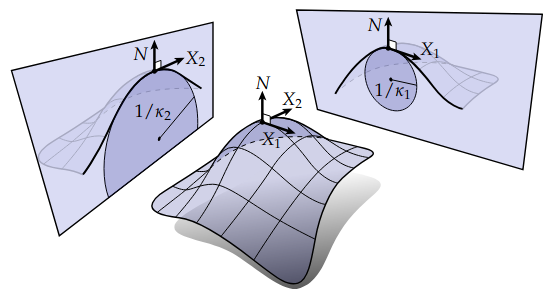
\includegraphics[width=0.7\textwidth]{../resources/principal_curvatures.png}
	% \includesvg[width=0.9\textwidth]{../resources/Minimal_surface_curvature_planes-en.svg}
	\caption{
Principal curvatures shown on an ellipsoidally round surface\cite{Digital_geom_proc_w_disc_ext_calc}.
$X_1$ and $X_2$ show the principal directions.
The curvature of a curve at a given point is the inverse of the radius of said curve.
The cutaway views show this as an osculated circle in each projection of the surface.
	}
	\label{fig:principal_k}
\end{figure}

There are however various ways of approximating the principal curvatures on a discrete mesh\cite{EstCurvOnTriMesh, DiscDiffGeoOpsTriMani}.
A basic approach is to calculate the mean and Gaussian curvatures, and derive the principal curvatures from them\cite{DDGAppIntro_19_discrete_k_2, Gauss_mean_k_notes}.
Given the mean curvature $H$ and Gaussian curvature $K$ (see \ref{sec:mean_k} and \ref{sec:gauss_k}), the principal curvatures can be calculated from \ref{eq:mean_k} and \ref{eq:gauss_k}.
\begin{align}
	\kappa_1 &= H - \sqrt{H^2 - K} \\
	\kappa_2 &= H + \sqrt{H^2 - K}
\end{align}
Although theoretically impossible, discretization errors can cause $H^2$ to be less than $K$, resulting in ``imaginary'' curvature.
This tends to occur on planar mesh regions, thus a minimum of 0 can be set for $H^2 - K$, because the root term would have been near 0 regardless, but it does highlight a flaw in this measure of curvature.

Taubin calculated the principal curvatures directly by estimating the tensor of curvature\cite{TaubinTensor}.
This has the benefit of direct calculation, but has been shown to be succeptible to noise in the mesh\cite{Comp_k_notes}.
Thiesel et al. calculate the curvature tensor per triangular face in the mesh, based on the face's corner normals\cite{Norm_based_k_tensor_est}.
Rusinkiewicz took a slightly different approach, calculating the curvature tensor for each mesh face via the differences between corner normals\cite{SRTensor}.
From there he computes the per vertex curvature tensor as a weighted sum over the curvature tensors of the vertex's adjoining triangles via coordinate system transformations.
Gatzke and Grimm examine a variety of other curvature estimation methods\cite{EstCurvOnTriMesh}, most of which were not considered for this work.

\subsection{Mean Curvature}\label{sec:mean_k}
Mean curvature is, as the name implies, the mean of the principal curvatures\cite{DDGAppIntro_19_discrete_k_2}:
\begin{equation}\label{eq:mean_k}
	H = \frac{\kappa_1 + \kappa_2}{2}
\end{equation}
Mean curvature can be approximated on a discrete mesh via sum of dihedral edge angle length products:
\begin{equation}\label{eq:dihedral_angle}
	H_i := \frac{1}{2}\sum_{j \in E}l_{ij} \phi_{ij}
\end{equation}
where $H_i$ is the mean curvature at vertex $i$, $j$ is a vertex in the ring of $i$, $l_{ij}$ is the length of the edge from $i$ to $j$, and $\phi_{ij}$ is the dihedral angle between the faces adjacent to edge $ij$.
See \ref{sfig:dihedral_angle} for a graphical depiction.

Alternatively, the mean curvature normal $\Delta f$ can be calculated via the discrete Laplace-Beltrami operator\cite{DDGAppIntro_18_discrete_k_1}:
\begin{equation}\label{eq:lap_beltrami_op}
	(\Delta f)_i := \frac{1}{2}\sum_{j \in E}(\cot \alpha_{ij} + \cot \beta_{ij})(p_j - p_i),
\end{equation}
and the absolute mean curvature can be calculated as half of the magnitude thereof:
\begin{equation}
	|H_i| = \frac{\|(\Delta f)_i \|}{2}.
\end{equation}
In equation \ref{eq:lap_beltrami_op} above $p_j$ is a vertex in the ring of vertex $p_i$ which indicates the current edge, $\alpha_{ij}$ and $\beta_{ij}$ are the angles opposite the current edge (see \ref{sfig:mesh_neighborhood}).

\begin{figure}[t]
	\centering
	\begin{subfigure}{0.45\textwidth}
		\centering
\begin{tikzpicture}[
	vertex/.style={circle, radius=2pt,fill, inner sep=2pt,outer sep=0pt},
	hidden/.style={inner sep=0, outer sep=0}]
	\node [vertex,label=180:i] (node_i) at (-0.4,2.2) {};
	\node [vertex,label=215:j] (node_j) at (0.4,-2.2) {};
	\node [hidden] (node_l) at (-2.3,-0.8) {};
	\node [hidden] (node_r) at (1.7,0.5) {};
	\draw (node_i) -- (node_j) -- (node_r) -- (node_i) -- (node_l) -- (node_j);
	\draw [dashed,gray!60] (node_l) -- (node_r);
	% try to draw curved arrow
	\draw [-Stealth,thick] (20:4mm) arc [start angle=20, delta angle=-180, x radius=5mm, y radius=3mm];
		% node [pos=0.8, label={250:$\phi_{ij}$}] {};
	\node [] at (-0.3, -0.6) {$\phi_{ij}$};
	\draw [|-|, thick] ($(node_i.east)+(0.1,0.05)$) -- ($(node_j.east)+(0.1,0.05)$)
		node [pos=0.65,label={0:$l_{ij}$}] {};
\end{tikzpicture}
		\caption{Dihedral angle of adjacent mesh faces. Inspired by \cite{DDGAppIntro_19_discrete_k_2}.}
		\label{sfig:dihedral_angle}
	\end{subfigure}
	\hfill
	\begin{subfigure}{0.45\textwidth}
		\centering
\begin{tikzpicture}[
	scale=1.1,
	vertex/.style={circle, radius=2pt,fill, inner sep=2pt,outer sep=0pt}]
	% based on image in slide 26/44 in DDG-DiscreteCurvatureI.pdf
	\newdimen\hexR
	\hexR=2cm
	\newlength\arcR
	\arcR=4mm
	\node[vertex,label=south west:i] (0, 0) {};
	\draw [thick] (330: \hexR) \foreach \x in {30,90,...,330} { -- (\x:\hexR) };
	\foreach \x in {30,90,...,330} {
		\draw (0, 0) -- (\x:\hexR) node[vertex]{};
	}
	% Vertex j
	\node [label=270:j] at (270:\hexR) {};
	\node [label=330:k] at (330:\hexR) {};
	% Inner main angle
	\draw (270:\arcR) arc [radius=\arcR, start angle=270, end angle=330]
		node [pos=0.5, label={[xshift=-3.5mm, yshift=1mm]300:$\Theta{ijk}$}] {};
	% Inner angles
	\draw (210:\hexR) +(330:\arcR) arc [radius=\arcR, start angle=-30, end angle=30]
		node [pos=0.5, label={[xshift=-2.2mm]0:$\alpha_{ij}$}] {};
	\draw (330:\hexR) +(150:\arcR) arc [radius=\arcR, start angle=150, end angle=210]
		node [pos=0.5, label={[xshift=2.5mm]180:$\beta_{ij}$}] {};
\end{tikzpicture}
		\caption{\raggedright The triangular mesh neighborhood around vertex $i$.}
		\label{sfig:mesh_neighborhood}
	\end{subfigure}
\caption{
(a) depicts two adjacent triangular faces connected by edge $ij$, with angle the dihedral angle between them denoted $\phi_{ij}$ and the length of edge $ij$ as $l_{ij}$.
(b) depicts the neighborhood of faces around vertex $i$ on some triangular mesh.
The angle between adjacent edges radiating from vertex $i$ is denoted $\Theta_{ijk}$.
The angles opposite edge $ij$ are indicated as $\alpha_{ij}$ and $\beta_{ij}$.
}
\end{figure}

\subsection{Gaussian Curvature}\label{sec:gauss_k}
Gaussian curvature\cite{TheoremaEgregium} is the product of the principal curvatures:

\begin{equation}\label{eq:gauss_k}
	K = \kappa_1 \cdot \kappa_2
\end{equation}

The discrete Gaussian curvature at a vertex is typically approximated as the ``angle defect'' divided by the vertex's area:
\begin{equation}
	K = \frac{2\pi - \sum \Theta_j}{A_i}
\end{equation}
where $\Theta_j$ is the angle between adjacent edges from the central vertex ($\Theta_{ijk}$ in \ref{sfig:mesh_neighborhood}), and $A_i$ is the vertex area.

Mean and Gaussian curvature are compared visually in figure \ref{fig:mean_gauss_k} from Pulla et al.
Note that the Gaussian curvature is approximately 0 over the entire surface, because the surface curves in only 1 direction, thus the 2nd principal curvature is ~0.
The colors shown in the mean curvature plot are effectively due entirely to the 1st principal curvature values.

\begin{figure}
	\centering
	% TODO: create a tikz picture to replace this image
	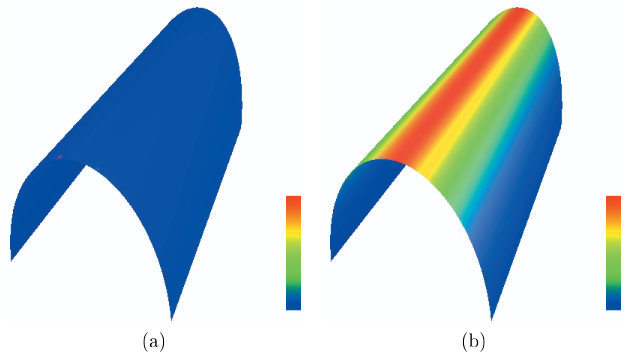
\includegraphics[width=0.9\textwidth]{../resources/gaussian_mean_k.png}
	\caption{Comparison of Gaussian (a) and mean (b) curvature\cite{Imp_k_estimation_for_WS}}
	\label{fig:mean_gauss_k} % NOTE: Label should be declared after caption
\end{figure}

\subsection{Root Mean Square Curvature}
Pulla et al. propsed using the root mean square curvature as the curvature estimate for use during watershed segmentation:
\begin{equation}
	\kappa_{rms} = \sqrt{\frac{\kappa_1^2 + \kappa_2^2}{2}}.
\end{equation}
They compared different measures of curvature for this purpose and found that it was approximately as good as absolute curvature:
\begin{equation}
	\kappa_{abs} = |\kappa_1| + |\kappa_2|,
\end{equation}
but cheaper to compute, because they computed $\kappa_{rms}$ from the mean and Gaussian curvatures using:
\begin{equation}
	\kappa_{rms} = \sqrt{4H^2 - 2K}.
\end{equation}
RMS curvature was used during developement prior to implementing the derivative of curvature.

\subsection{Derivative of Curvature}
Through testing it was determined that supplying the derivative of curvature instead of the curvature itself to watershed segmentation would better preserve the boundaries between semantic regions.
Rusinkiewicz proposes a method of taking the derivative of the curvature tensor\cite{SRTensor}.
Because watershed segmentation expects a single value rather than a tensor, the magnitude of the derivative of the curvature tensor was approximated as the sum of squares of said tensor.

\section{UV Mapping}
UV Mapping is the process of projecting a surface from 3D to 2D, effectively ``unwrapping'' the 3D surface.
(insert sentence about common usage in 3D modeling / graphics and textures)
The UV map for planar surfaces is trivial, as the 3D surface is already ``unwrapped''.

\subsection{Conic Surfaces}
General equation of a conic is:
\begin{equation}\label{eq:gen_conic}
	Ax^2 + Bxy + Cy^2 + Dx + Ey + F = 0
\end{equation}

\subsubsection{Elliptic Surface}
General equation:
\begin{equation}
	\frac{x^2}{a^2} + \frac{y^2}{b^2} = 1
\end{equation}
To obtain a vector perpendicular to a point on the ellipse, the derivative of said point is rotated 90 degrees.
The point, as a function of the angle $\theta$:
\begin{equation}
	(x,y) = (a\cos\theta, b\sin\theta)
\end{equation}
The derivative thereof:
\begin{equation}
	\frac{d}{d\theta}(x,y) = (-a\sin\theta, b\cos\theta)
\end{equation}
Rotated -90 degrees:
\begin{equation}
	\text{Rot}_{90}\frac{d}{d\theta}(x,y) = (b\cos\theta, a\sin\theta)
\end{equation}

\subsubsection{Parabolic Surface}
Parabolas are much simpler than and ellipses and hyperbolas, as can be seen by the following equations.
The parametric general equation of a parabola is:
\begin{equation}
	-\sin\theta x + \cos\theta y = \frac{1}{4f}(\cos\theta x + \sin\theta y - h)^2 + k
\end{equation}
To solve for the conic parameters of a parabola the general equation's quadratic term is expanded and like terms gathered:
\begin{multline*}
	-\sin\theta x + \cos\theta y = \frac{1}{4f}(\cos^2\theta x^2 + \cos\theta\sin\theta xy \\
	- h \cos\theta x + \cos\theta\sin\theta xy + \sin^2\theta y^2 - h\sin\theta y - h \cos\theta x - h \sin\theta y + h^2) + k
\end{multline*}
\begin{multline*}
	\frac{\cos^2\theta}{4f} x^2 + \frac{2\cos\theta\sin\theta}{4f} xy + \frac{\sin^2\theta}{4f} y^2 \\
	+ \left(\sin\theta - \frac{2h \cos\theta}{4f}\right)x + \left(\cos\theta - \frac{2h \sin\theta}{4f}\right)y + \frac{h^2}{4f} + k = 0
\end{multline*}
\begin{align}
	A &= \frac{\cos^2\theta}{4f} \\
	B &= \frac{2\cos\theta\sin\theta}{4f} \\
	C &= \frac{\sin^2\theta}{4f} \\
	D &= \sin\theta - \frac{2h \cos\theta}{4f} \\
	E &= \cos\theta - \frac{2h \sin\theta}{4f} \\
	F &= \frac{h^2}{4f} + k
\end{align}

\subsubsection{Hyperbolic Surface}
\begin{equation}
\begin{split}
	\frac{(\cos\theta(x-h) + \sin\theta(y-k))^2}{a^2} - \frac{(\cos\theta(y-k) + \sin\theta(x-h))^2}{b^2} &= 1 \\
	\frac{(x_c + y_s)^2}{a^2} - \frac{(y_c + x_s)^2}{b^2} &= 1 \\
	b^2(x_c^2 + 2x_c y_s + y_s^2) - a^2(y_c^2 + 2 x_s y_c + x_s^2) &= a^2 b^2 \\
	b^2 x_c^2 + 2 b^2 x_c y_s + b^2 y_s^2 - a^2 y_c^2 - 2 a^2 x_s y_c - a^2 x_s^2 - a^2 b^2 &= 0 \\
	b^2 x_c^2 - a^2 x_s^2 + 2 b^2 x_c y_s - 2 a^2 x_s y_c + b^2 y_s^2 - a^2 y_c^2 - a^2 b^2 &= 0 \\
\end{split}
\end{equation}
\begin{multline*}
	b^2 (\cos\theta(x-h))^2 - a^2 (\sin\theta(x-h))^2 \\
	+ 2 b^2 \cos\theta(x-h) \sin\theta(y-k) - 2 a^2 \sin\theta(x-h) \cos\theta(y-k) \\
	+ b^2 (\sin\theta(y-k))^2 - a^2 (\cos\theta(y-k))^2 - a^2 b^2 = 0
\end{multline*}
\begin{multline*}
	(b^2 \cos^2\theta - a^2 \sin^2\theta)(x-h)^2 \\
	+ 2 \cos\theta\sin\theta(b^2 - a^2)(x-h)(y-k) \\
	+ (b^2 \sin^2\theta - a^2 \cos^2\theta)(y-k)^2 - a^2 b^2 = 0
\end{multline*}
\begin{equation*}
	\begin{split}
		c_1(x-h)^2 + c_2(x-h)(y-k) + c_3(y-k)^2 - a^2 b^2 &= 0 \\
		c_1(x^2-2hx + h^2) + c_2(xy-hy-kx+hk) + c_3(y^2-2ky+k^2) - a^2 b^2 &= 0 \\
		c_1 x^2 + c_2 xy + c_3 y^2 + (-2h c_1 -k c_2) x + (-h c_2 -2k c_3)y + c_1 h^2 + c_2 hk + c_3 k^2 - a^2 b^2 &= 0 \\
	\end{split}
\end{equation*}
\begin{align*}
	A &= c_1 = b^2 \cos^2\theta - a^2 \sin^2\theta \\
	B &= c_2 = 2 \cos\theta\sin\theta(b^2 - a^2) \\
	C &= c_3 = b^2 \sin^2\theta - a^2 \cos^2\theta \\
	D &= (-2h c_1 -k c_2) \\
	E &= (-h c_2 -2k c_3) \\
	F &= c_1 h^2 + c_2 hk + c_3 k^2 - a^2 b^2
\end{align*}
Now to solve for $a$, $b$, and $\theta$:
Solving $A$ for $b^2$:
\begin{equation}
	\begin{split}
		A &= b^2 \cos^2\theta - a^2 \sin^2\theta \\
		b^2 &= \frac{A}{\cos^2\theta} + a^2\tan^2\theta \\
	\end{split}
\end{equation}
Setting 3.6 into $C$ and solving for $a^2$:
\begin{equation}
	\begin{split}
		C &= b^2 \sin^2\theta - a^2 \cos^2\theta \\
		a^2 &= -\frac{C}{\cos^2\theta} + b^2\tan^2\theta \\
		a^2 &= -\frac{C}{\cos^2\theta} + \left(\frac{A}{\cos^2\theta} + a^2\tan^2\theta\right)\tan^2\theta \\
		\cos^4\theta a^2 &= -C\cos^2\theta + A\cos^2\theta + \sin^4\theta a^2 \\
		(\cos^4\theta - \sin^4\theta) a^2  &= \cos^2\theta(A-C) \\
		a^2  &= \frac{\cos^2\theta(A-C)}{(\cos^4\theta - \sin^4\theta)} \\
	\end{split}
\end{equation}
Setting 3.6 into $B$:
\begin{equation}
	\begin{split}
		B &= 2 \cos\theta\sin\theta(\frac{A}{\cos^2\theta} + a^2\tan^2\theta - a^2) \\
		\cos^2\theta B &= 2 \cos\theta\sin\theta(A + (\sin^2\theta - \cos^2\theta) a^2) \\
	\end{split}
\end{equation}
Setting 3.7 into 3.8:
\begin{equation}
	\begin{split}
		\cos^2\theta B &= 2 \cos\theta\sin\theta(A + (\sin^2\theta - \cos^2\theta) \frac{\cos^2\theta(A-C)}{(\cos^4\theta - \sin^4\theta)}) \\
	\end{split}
\end{equation}

\section{Ramer-Douglas-Peucker Algorithm}
The Ramer-Douglas-Peucker (RDP) algorithm is a method to interatively simplify a line defined by a set of points.
The only arguments to RDP are a list of points and a tolerance width, within which points will be considered unnecessary and discarded.
% The algorithm looks at a list of points, draws an imaginary line from the first to the last, finds the point with the farthest normal distance to the comparison line, and if the point's distance to the comparison line is greater than a pre-defined tolerance width, splits the lin
The algorithm iteratively finds the point farthest from the straight line from point 0 to n-1, and if said distance is greater than the tolerance width, the line is split at the farthest point and the line sections before and after the split are reconsidered individually.
The procedure is described in greater detail in algorithm \ref{alg:RDP}.

\begin{algorithm}[H]
\caption{Ramer-Douglas-Peucker}\label{alg:RDP}
\begin{algorithmic}[1]
\Function{SimplifyLineRDP}{points $P$, real $w$}
	\State new list $P_{core}$\Comment{To store the important point indices}
	\State new RDPNode $n_0 \leftarrow$ RDPNode($P$.first, $P$.last)
	\State new list $N_{stack} \leftarrow n_0$
	\While{$N_{stack}$ not empty}
		\State new RDPNode $n \leftarrow N_{stack}$.last
		\State $N_{stack}$.popLast()
		\State new uint $i \leftarrow$ index of point farthest from $n$.line
		\State new real $d \leftarrow$ distance of $P$[$i$] from $n$.line
		\If{$d \le w$} \Comment{If farthest point is within tolerance}
			\State $P_{core}$.append($n$.srcPt) \Comment{line section is complete}
			\State \textbf{continue}
		\EndIf
		\State new RDPNode $n_{left} \leftarrow$ RDPNode($n$.srcPt, $P$[$i$])
		\State new RDPNode $n_{right} \leftarrow$ RDPNode($P$[$i$], $n$.endPt)
		\State $N_{stack}$.append($n_{right}$)
		\State $N_{stack}$.append($n_{left}$)
	\EndWhile
	\State $P_{core}$.append($P$.last)
	\State \textbf{return} $P_{core}$
\EndFunction
\end{algorithmic}
\end{algorithm}

The RDP implementation used in this work uses a struct \textbf{RDPNode} that represents a section of the line.
It contains a start and end point, as well as a line spanning these two points.
A stack is used to manage the \textbf{RDPNode}s.
In each iteration of the \verb|while| loop, starting on line 5, the item at the top of the stack is removed and stored in $n$.
The point farthest from this line section is found, and on line 10 the distance thereof is compared against the tolerance width.
If the perpendicular distance is within the tolerance width then the current line section is complete and the initial point in the section is added to $P_{core}$ (line 11).
If not, then the current line section is split at the farthest point, with the two new sections represented by RDPNodes $n_{left}$ and $n_{right}$.
These are then placed on the stack, $n_{right}$ first, so that $n_{left}$ is processed next, ensuring the list of important points $P_{core}$ is always sorted.
After the \textbf{RDPNode} stack is exhausted the last point in $P$ is appended to $P_{core}$ because only the start point in each node is added to $P_{core}$.
An alternative implementation that uses recursion may be found on wikipedia.

\section{Traveling Salesman Problem}
The Traveling Salesman Problem (TSP) is a well known problem in combinatorial optimization.
The original problem was posed as the following:
A salesman wishes to visit every city in a given region once, to spend the least amount of time traveling between cities, and to end at his home city.
It was initially formulated in the 1800s by mathematicians William Rowan Hamilton and Thomas Kirkman\cite{Graph_theory}.
The problem can be stripped down to simply the optimal round-trip traversal of a set of nodes in a graph, where the traversal represents the salesman's movement, and each node represents a city.
It can be shown\cite{TSP_in_pursuit_of} that for $n$ nodes the number of possible route permutations is
\begin{equation*}
	n_{\text{routes}} = (n-1)!.
\end{equation*}
For the vast majority of applications symmetric node-to-node costs can be assumed, and the number of permutations is reduced to \textit{only}
\begin{equation*}
	n_{\text{routes}} = \frac{(n-1)!}{2}.
\end{equation*}
The number of real world TSP applications is similarly large\cite{TSP_theory_applications}, ranging from determining the drill order of holes in printed circuit board manufacturing\cite{TSP_PCB_manufacturing}, to mail delivery and vehicle routing in general\cite{TSP_mail_delivery}, to X-ray crystallography\cite{TSP_xray_crystallography}.
The algorithm described in this work produces a set of convex surfaces from the target object.
Within each convex surface region a simple path is planned.
% NOTE the verb tense/case! "would" because it is not implemented
It is the traversal of these surface regions that would be formulated as a TSP with the distance between each region and the change in end-effector orientation serving as the travel costs.
Considering only the traversal of the surface regions, the start and end nodes need not be the same, and the situation can be modeled as a modified TSP.
The common way to modify a TSP to achieve different start and end nodes is to introduce a dummy node with 0-cost edges to the other nodes\cite{TSP_dummy_node_mod}.
After insertion of the dummy node, the TSP can be solved like normal.
Once the TSP has been solved the nodes adjacent to the dummy node are the start and end nodes.
If the robot's starting or home position is included as a node, the application can be handled as a classic TSP.



%! TeX root = thesis.tex
\chapter{Methodology}\label{methodology}
\IMRADlabel{methods}

\section{Overview}
The basic premise is to segment the given model into primitive surfaces.
Each surface is unwrapped to a 2D representation, which undergoes a 2D segmentation to produce convex regions.
Upon each convex region a local path is planned.
The order in which each region is traversed by the robot is determined via a modified Traveling Salesman Problem.
Here, the start and end points of the salesman's path need not be the same.

\section{3D Segmentation}
Segmentation in 3D consists of breaking the model into primitive surfaces,
which have (easily) solvable mappings from 3D to 2D.
This is done by applying Watershed segmentation to the mesh as a whole and classifying the resultant mesh sections as a certain primitive.
Watershed segmentation is imperfect, and sometimes yields mesh sections comprised of multiple primitive types.
In such cases the composite mesh section undergoes Watershed segmentation again, but with a lower merge threshold (see \ref{ws_seg}), so that it might be split into multiple mesh sections.

$\rightarrow$ Do i need to further describe Seg3D ?

\subsection{Watershed Segmentation}\label{ws_seg}
A watershed, according to the North American usage, is an area of land, in which all streams and rainfall drain to a common body of water\cite{USGS_Watersheds}, also commonly called catchment basins.
Somewhat confusingly, the rest of the English speaking world uses ``Watershed'' to refer to the high elevation regions that separate said catchment basins.
Watershed segmentation originally comes from image processing, where it is used for image segmentation\cite{ImageSegWS, DigitalImageProc}.
It works by applying a ``height function'' to the input image and forming image regions divided by ``high'' areas.
A common ``height function'' in image processing is the gradient of the image\cite{ImageSegWS}.
Mangan and Whitaker first applied this concept to 3D meshes, replacing pixels for the mesh's vertices and the image gradient for the mesh curvature\cite{Watershed}.

-> Give overview of how WS segmentation works.
\subsubsection{Basic Procedure}
Their algorithm consists of 6 steps:
\begin{enumerate}
	\item Apply the height function to each vertex
	\item Find and label each local minima
	\item Find flat areas and classify them as either a minimum or plateau
	\item Loop through the plateaus and allow each to descend to a labeled region
	\item Descend from all remaining vertices to labeled regions
	\item Merge regions whose watershed depth is below a given threshold
\end{enumerate}

0. Apply height function at each vertex
1. Create initial mesh regions from local minima / minima plateaus
2. ``Minima Expansion'' Expand outward from each mesh region up to a certain depth, absorbing any regions encountered.
3. ``Descent to Minima'' From each un-indexed (check their word for this) vertex, follow the path of steepest descent until an indexed region is encountered.
All vertices traversed along this descent are added to the encountered region.

-> my modifications
\subsubsection{Mini-Merge}
As noted by Mangan and Whitaker(sp?) Descent to Minima will segment the given mesh, but in all likelihood it will be overly segmented.
Through testing small high curvature regions were observed, that due to their high curvature did were not merged into any of the larger more useful regions.
To combat this, the ``Mini Merge'' step was developed to merge regions deemed too small to be worth keeping.

\subsubsection{Boundary Smoothing}
This step is more post-processing and ``cleaning'' of the mesh region boudnary than actual segmentation.
Due to randomness in the mesh there are situations where a vertex is connected to its region by a single edge.
Such vertices are named ``web1'' points, due to them having a single webbed connection to their region's perimeter.
In order to smooth the region boundary, an attempt is made to find an adjacent mesh region more suitable to possess each web1 point.
Because vertices with only 3 edges are exceedingly rare in well meshed models, it is sufficient to transfer ownership of the web1 point to the adjacent region with the highest number of connecing edges.
Thus, for example, A vertex assigned to region 4 through Minima Descent with edges connecting to regions 4, 10, 12, and 12, would be transferred to region 12.
No explicit tie breaking mechanism was deemed necessary, but lower numbered regions are likely given priority due to how the code was written.
TODO: Need to check what other cases could occur...

\subsection{Surface Classification}

\section{Geometry Simplification}
GeoSimp creates simplified geometric representations of the 3D mesh sections it is given

\subsection{Shared Edges}
see \verb|create_shared_edges()|

\subsection{Shared Corners}

\subsection{Simplified Surfaces}

\section{2D Segmentation}
This is Interior Edge Extension
The idea was that downstream components requried convex shapes to facilitate local path planning.
In hindsight, surfaces need not be completely convex, but merely \textit{mostly} convex.

\section{Surface Path Planning}
This is effectively Boustrophedon

\section{Modified Traveling Salesman Problem}
Normal TSP should have already been described in \ref{background}, so no need to rehash that.
Only need to talk about the modifications and how it would have been applied...

\section{Inverse Kinematics}
Talk about how the InvKin from the robot could be used, but a custom one would (likely) be necessary to incorporate the rotary table



%! TeX root = thesis.tex
\chapter{Results}
\IMRADlabel{results}
Describe results here...


%! TeX root = thesis.tex
\chapter{Discussion}
\IMRADlabel{discussion}
Discussion! did it work?

\section{Watershed Segmentation}
Watershed segmentation as implemented here, functioned as intended.
Based on the results observed, the cause of any segmentation issues is believed to lie with the height function chosen.
Though not thoroughly tested, the Watershed modifications made in this work are expected to have been non-detrimental.
(? probably better without the previous sentence...)
% There is no reason to believe the additions / modifications / implementation here is responsible for the issues encountered.

\section{Surface Classification}
Of the implemented primitives, plane and elliptic cylinder, surface classification works as intended.
Expanding this project to handle the third proposed primitive, ellipsoids, would be relatively straightforward, given that Eberly's work on ellipses extends to ellipsoids~\cite{GeoTools_pt_to_ellipse}.
Should the approach of primitive segmentation and classification be pursued further, the functionality to handle more primitives will be necessary.
Beyond ellipsoids, the main remaining geometric primitives are the cone and torus.
For both of these Eberly once again offers solutions~\cite{GeoTools_least_squares_fitting}, though fitting a cone to 3D points can likely be simplified by exploiting the input mesh's normals.
% The surface classification methods presented here, although they represent earnest attempts, are generally unreliable. -> less so since classifiers were replaced with pure regression.

\section{2D Segmentation}
The stated goals of the \textit{interior edge extension}\cite{IntEdgeExt} are:
\begin{enumerate}
	\item to minimize the number of changes in direction of the planned paths.
		This goal leads to the optimization requirement of minimizing the sum of cell widths when solving the weighted set coverage problem.
	\item to produce convex cells.
\end{enumerate}

Minimizing the number of direction changes is of value if the cost in time or energy of a direction change is non-negligible, as is the case for mobile robots such as automated agriculture machines, AUVs, and to a lesser degree UAVs.
However the cost of direction change for a robot arm is minimal.
Furthermore, the envisioned end-effector tool is equally effective in its surface treatment moving in the positive or negative direction normal to the laser plane.
(? rethink previous sentence...?)
That is, while a Roomba would be less effective if it were to traverse its environment backwards, the laser module suffers no such loss of efficacy.
% a ``planar laser'' (? revisit with better wording)
% need not rotate at each switchback because it is
Hence, the goal of minimzing the number of switchbacks was unnecessary for this work.

Nielsen et al. do not explain why the final polygons should be convex, treating it as a given.
Boustrophedon path planning requires cells to be \textit{semi}-convex, not necessarily truly convex.
This is illustrated in Figure \ref{fig:bpath_semi_convex} below.

\begin{figure}[htb]
	\centering
	\begin{tikzpicture}[scale=1.0]
		\datavisualization[
			% new Cartesian axis=x axis, x axis={attribute=x},
			% new Cartesian axis=y axis, y axis={attribute=y},
			scientific axes,%=clean,
			all axes={ticks={major={at={}},minor={at={}}}},
			data/format=table,
			% yticklabel={\empty},
			% school book axes,
			visualize as line/.list={outline,path},
			% /data point/set/outline/.initial=1
			% outline={style={}},
			path={style={red}}
			]
			data[
				headline={x,y},
				read from file="../resources/boustrophedon/ex_2_polygon.csv",
				set=outline]
			data[
				headline={x,y},
				read from file="../resources/boustrophedon/ex_2_path.csv",
				set=path];
	\end{tikzpicture}
	\caption{Boustrophedon path planning performed on a semi-convex shape}
	\label{fig:bpath_semi_convex}
\end{figure}

For semi-convex polygons the sweep direction may no longer be chosen based on the longest edge.
The sweep direction must be chosen such that a line parallel to the sweep direction reaches the entire polygon when swept along the shift direction.
% A formal definition of ``semi-convex'' is beyond the scope of this work, and left for future work, but ..?
Although a formal definition of ``semi-convex'' is beyong the scope of this work, an informal one may be attempted (? approached).
% This is best described with an image, see below.

\subsection{Isovist Line}
% TODO: new name... "bivist line" ?
To define a useful measure of "semi-convexity" the notion of the isovist is helpful.
Benedikt gives the definition of an isovist as "the set of all points visible from a given vantage point in space and with respect to an environment"\cite{Isovists}.
While the isovist concept is primarily used in architecture and urban spaces, it can also be applied to computational geometry.
In the \textit{art gallery problem} each guard represents an isovist, and the solution to a given art gallery problem is the minimum number of isovists to completely cover the given environment.
A similar problem in computational geometry is the \textit{watchman route problem}, in which the a single mobile watchman is tasked with guarding an environment with obstacles.
The challenge lies in determining the shortest path the watchman should take to observe the entire environment.
Determining a polygon's ``semi-convexity'' draws on both of these problems by reducing the number of guards is to one, whose scope of observation is further reduced to a single line in both directions, but who \textit{is} allowed to move perpendicular to the viewing direction.
% Extending the art gallery problem to create a semi-convexity-test for a polygon, the number of guards is reduced to one, whose scope of observation is further reduced to a single line in both directions, but who \texti{is} allowed to move perpendicular to the viewing direction.
If ``guarding'' the polygon this way is feasible, then the polygon is at least semi-convex, and boustrophedon path planning may be applied, with the shift direction set to the guard's direction of movement, and the sweep direction perpendicular thereto.
Naturally, convex polygons pass this test as well.
% Each guard is reduced to looking along a single line in both directions, but is allowed to move along a line perpendicular to the viewing direction.

\section{Cellular Path Planning}
Cellular path planning using boustrophedon path planning worked as expected.
There was potential for expansion, such as allowing the TSP to potentially determine the path start point on the polygon.
This is left for a future expansion of the project, in which the TSP is fully implemented.



\chapter{Conclusion}
% This is what it /can/ do well, and /this/ is where it falls short.
This project, or at a minimum the overall concept chosen, proved more arduous than anticipated and requiring more time than available.
The complete pipeline is capable of processing models with planar surfaces.
At the time of writing, corners where four or more edges converge cause issues, and should be avoided if possible.
(? Given a few extra days, fixing this should be easily possible.)
As for curved surfaces, concave curves will at a minimum cause oversegmentation during the \textit{2D Segmentation} step, as discussed in the previous chapter.
The procedure is also unable to properly handle convex curves, but would require less effort to finish that functionality.
Furthermore, smooth transitions between primitive types constitute another open challenge.

Throughout development great emphasis was placed on reaching a point where the program and procedure could be tested in its entirety, and imroved from there.
In hindsight, this approach to development was ill-suited to a project of this nature, where the main building blocks are each complex and somewhat fragile.
If the time had been taken to test and refine \textit{Watershed Segmentation} and \textit{Surface Classification} to maturity, the issue regarding the height function selection could have been detected early enough to solve within the bounds of this project.

% Current conclusion(s):
% \begin{enumerate}
% 	\item I did not do sufficient research in the beginning, leading to wasted efforts later on
% 	\item My workflow was short-sighted, in that i only thought / considered a few steps ahead of my current position, rather than having a solid "big picture" view
% 	\item For simple flat objects with sharp edges, it works fine
% 	\item ...?
% \end{enumerate}

% I suggest /not/ continuing without serious reconsideration of either the objectives or the overall concept.
A continuation of this project without serious reevaluation of the overall concept is strongly disadvised.
The geometric primitive segmentation and classification concept is likely to be too rigid to effectively handle truly ``arbitrary'' geometry.
Should the range of the project's input geometry be restricted in future iterations, then this concept may prove viable.

\section{Outlook}
There are plenty of aspects of this project that could be improved.
These range from mere bug-fixes to replacing entire algorithms.
If the project were to be continued with all high-level components and steps, \textit{Interior Edge Extension} would require more testing to improve its robustness and fix minor bugs.

In order to maintain the current concept while allowing high-level and algorithm changes, the following improvements are recommended.

Further work would include:
\begin{itemize}
	\item An approach to handle both ``hard'' \textit{and} ``soft'' edges must be developed.
	\item Implement regression and classification functions for remaining geometric primitives
	\item \textit{Geometry Simplification} should be expanded and improved to solve the aforementioned shortcomings, and to improve robustness.
	\item The \textit{Interior Edge Extension} step should be replaced with one better suited to shapes with curved edges.
		The Boustrophedon Cellular Decomposition or an expansion thereof would provide a decent starting point for its replacement.
	\item The Traveling Salesman Problem should be implemented to join the individual cellular paths.
	% \item Inverse kinematics that better take into account the rotary table
	% \item Reachability was basically ignored in this project, so that should be explored...
	\item Reachability of the poses generated by the path planner will need to be taken into account before the procedure may be used outside of a test environment.
\end{itemize}



\appendix

%! TeX root = thesis.tex
\chapter{Test Objects}\label{App:model_table}

The following are the 3D models used to test the program.
The values listed under `source' have the following meanings:
\begin{itemize}
	\item \textbf{GC-PF}: Model downloaded from GrabCAD created by user paulocferreira 3D\cite{GC-PF}.
		User paulocferreira 3D numbers their basic models, which makes finding the source for a given model fairly straightforward.
		A specific model can be found by finding the model that corresponds to the number from the ID of a \textbf{GC-PF} sourced model: \verb|fcXXX|.
	% \item \textbf{GC-[A]}: Model was downloaded from GrabCAD, created by user XXX
	\item \textbf{10k}: Model downloaded from Thinki10k, a database of 3D models\cite{Thingi10k_paper, Thingi10k_app}.
		To find the specific webpage for a given model, replace \verb|XXX| in \verb|https://ten-thousand-models.appspot.com/detail.html?file_id=XXX| with the ID from the table.
	\item \textbf{Thing}: Model downloaded from Thingiverse.
		Specific Thingiverse webpages can be found by replacing the \verb|XXX| in \verb|https://www.thingiverse.com/thing:XXX| with the ID from the table.
\end{itemize}

\csvreader[%
	longtable = |lcccl|,
	respect underscore = true,
	table head = \hline
	\textbf{ID} &
	\textbf{Source} &
	\textbf{Mesh} &
	\textbf{Class} &
	% \textbf{Explanation} &
	\textbf{Outcome}\\\hline\hline,
	late after line = \\\hline,
	late after last line = \\\hline
]{../resources/model_table.csv}{
	Filename=\id,
	% Description=\desc,
	Source=\src,
	Mesh=\mesh,
	Class=\class,
	% Reason=\reason,
	Outcome=\outcome
} {% Comment to prevent first couple lines from being shifted right slightly
	\id & \src & \mesh & \class & \outcome
}% https://tex.stackexchange.com/a/619232



\printbibliography

\end{document}
